\FloatBarrier
\subsection{Under \& Over parameterization}
Our evaluation of under- and overparameterized systems is based on the model with white noise input and colored noise output. The necessary $\phi$ matrices for the underparameterized and overparameterized systems are defined in \autoref{eq:LSIUOPUnderPPhi} and \autoref{eq:LSIUOPOverPPhi}, respectively. Note that some matrix indexing was adjusted to ensure proper code execution.

\begin{equation}
	phi = [-y(2:N-1)'; -y(1:N-2)'; u(2:N-1)'; u(1:N-2)'];
	\label{eq:LSIUOPUnderPPhi}
\end{equation}


\begin{equation}
	\begin{aligned}
	phi = &[-y(4:N-1)'; -y(3:N-2)'; -y(2:N-3)'; -y(1:N-4)';\\
	 &u(4:N-1)'; u(3:N-2)'; u(2:N-3)'; u(1:N-4)'];
	\end{aligned}
	\label{eq:LSIUOPOverPPhi}
\end{equation}


\autoref{fig:LSIUOPUnderPOutputVSSimulated} and \autoref{fig:LSIUOPOverPOutputVSSimulated} represet the output of under and overparameterized system versus the simulated output for each of them accordingly. The resulting transfer function for underparameterized system is shown in \autoref{eq:LSIUOPUnderP} and the transfer function of overparameterized system is displayed in \autoref{eq:LSIUOPOverP}. On average the resulted MSE for underparameterized is worse than a system with proper amount of parameters. The overparameterized system probably overfits the provided data and eventhough it is performing better on test data, it is not generalized and will not really mirror the actual system outputs if implemented in a real world scenario.

\begin{figure}
\centering
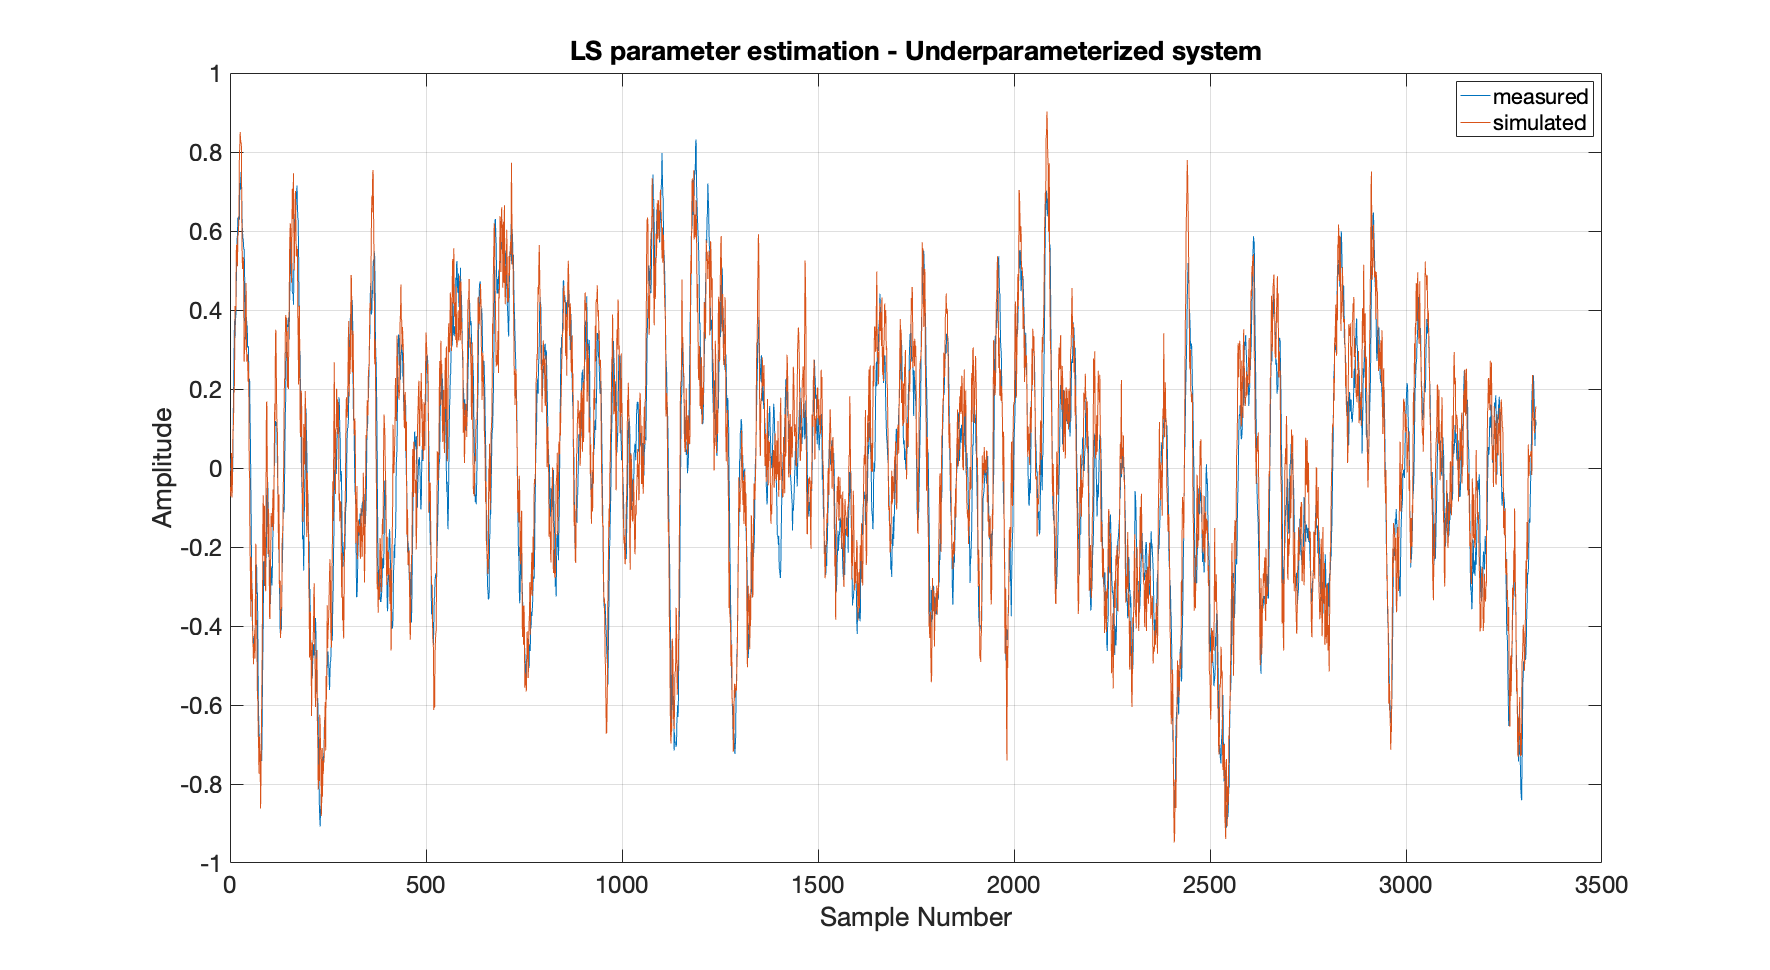
\includegraphics[totalheight=8cm]{images/LSIUOPUnderPOutputVSSimulated.png}
\caption{LS underparameterized system output comparison for colored noise on output}
\label{fig:LSIUOPUnderPOutputVSSimulated}
\end{figure}

\begin{equation}
	G(z) =	\frac{0.04284 z + 0.01567}{z^2 - 0.9191 z - 0.04081}
	\label{eq:LSIUOPUnderP}
\end{equation}

\begin{figure}
	\centering
	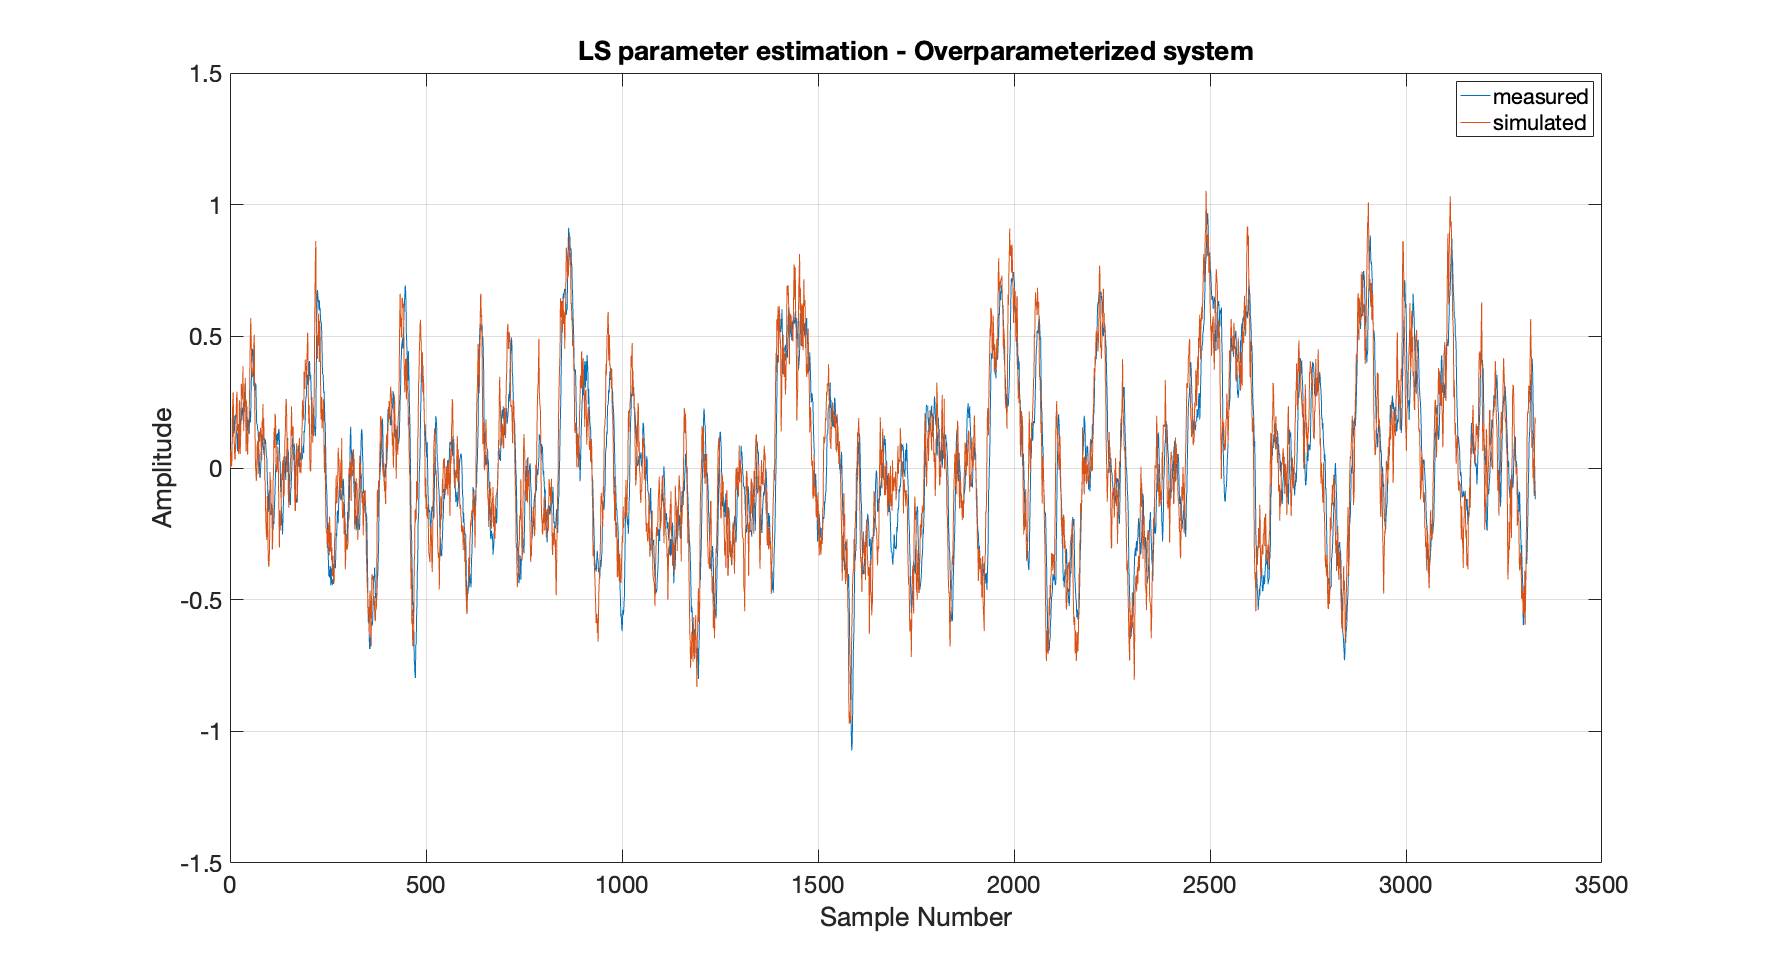
\includegraphics[totalheight=8cm]{images/LSIUOPOverPOutputVSSimulated.png}
	\caption{LS overparameterized system output comparison for colored noise on output}
	\label{fig:LSIUOPOverPOutputVSSimulated}
\end{figure}

\begin{equation}
	G(z) =	\frac{0.04464 z^3 + 0.01715 z^2 + 0.01449 z + 0.01368}{z^4 - 0.8713 z^3 - 0.02817 z^2 - 0.03509 z - 0.013}
	\label{eq:LSIUOPOverP}
\end{equation}

The implemented Matlab code for underparameterized system is located at  \hspace{-1ex}\lstinline| assignment1/part1/1_4/LS1_4_under.m| and the code for overparameterized system is located at  \hspace{-1ex}\lstinline| assignment1/part1/1_4/LS1_4_over.m| . 
